% Options for packages loaded elsewhere
\PassOptionsToPackage{unicode}{hyperref}
\PassOptionsToPackage{hyphens}{url}
\documentclass[
  11pt,
  a4paper,
]{scrartcl}
\usepackage{xcolor}
\usepackage[top=23mm,bottom=23mm,left=24mm,right=24mm]{geometry}
\usepackage{amsmath,amssymb}
\setcounter{secnumdepth}{-\maxdimen} % remove section numbering
\usepackage{iftex}
\ifPDFTeX
  \usepackage[T1]{fontenc}
  \usepackage[utf8]{inputenc}
  \usepackage{textcomp} % provide euro and other symbols
\else % if luatex or xetex
  \usepackage{unicode-math} % this also loads fontspec
  \defaultfontfeatures{Scale=MatchLowercase}
  \defaultfontfeatures[\rmfamily]{Ligatures=TeX,Scale=1}
\fi
\usepackage{lmodern}
\ifPDFTeX\else
  % xetex/luatex font selection
\fi
% Use upquote if available, for straight quotes in verbatim environments
\IfFileExists{upquote.sty}{\usepackage{upquote}}{}
\IfFileExists{microtype.sty}{% use microtype if available
  \usepackage[]{microtype}
  \UseMicrotypeSet[protrusion]{basicmath} % disable protrusion for tt fonts
}{}
\usepackage{setspace}
\makeatletter
\@ifundefined{KOMAClassName}{% if non-KOMA class
  \IfFileExists{parskip.sty}{%
    \usepackage{parskip}
  }{% else
    \setlength{\parindent}{0pt}
    \setlength{\parskip}{6pt plus 2pt minus 1pt}}
}{% if KOMA class
  \KOMAoptions{parskip=half}}
\makeatother
\usepackage{longtable,booktabs,array}
\newcounter{none} % for unnumbered tables
\usepackage{calc} % for calculating minipage widths
% Correct order of tables after \paragraph or \subparagraph
\usepackage{etoolbox}
\makeatletter
\patchcmd\longtable{\par}{\if@noskipsec\mbox{}\fi\par}{}{}
\makeatother
% Allow footnotes in longtable head/foot
\IfFileExists{footnotehyper.sty}{\usepackage{footnotehyper}}{\usepackage{footnote}}
\makesavenoteenv{longtable}
\usepackage{graphicx}
\makeatletter
\newsavebox\pandoc@box
\newcommand*\pandocbounded[1]{% scales image to fit in text height/width
  \sbox\pandoc@box{#1}%
  \Gscale@div\@tempa{\textheight}{\dimexpr\ht\pandoc@box+\dp\pandoc@box\relax}%
  \Gscale@div\@tempb{\linewidth}{\wd\pandoc@box}%
  \ifdim\@tempb\p@<\@tempa\p@\let\@tempa\@tempb\fi% select the smaller of both
  \ifdim\@tempa\p@<\p@\scalebox{\@tempa}{\usebox\pandoc@box}%
  \else\usebox{\pandoc@box}%
  \fi%
}
% Set default figure placement to htbp
\def\fps@figure{htbp}
\makeatother
\setlength{\emergencystretch}{3em} % prevent overfull lines
\providecommand{\tightlist}{%
  \setlength{\itemsep}{0pt}\setlength{\parskip}{0pt}}

\usepackage{microtype}
\usepackage{xcolor}
\usepackage{needspace}
\definecolor{linkink}{HTML}{553653}
\AtBeginDocument{\hypersetup{colorlinks=true,linkcolor=linkink,urlcolor=linkink,citecolor=linkink}}
\setlength{\emergencystretch}{3em}
\setlength{\parindent}{0pt}
\setlength{\parskip}{0.42em}
\widowpenalty=10000
\clubpenalty=10000
\displaywidowpenalty=10000
\allowdisplaybreaks[1]
\usepackage{bookmark}
\IfFileExists{xurl.sty}{\usepackage{xurl}}{} % add URL line breaks if available
\urlstyle{same}
\hypersetup{
  pdftitle={Algebraic extinction in acyclic compartment models},
  pdfauthor={Anonymous},
  hidelinks,
  pdfcreator={LaTeX via pandoc}}

\title{Algebraic extinction in acyclic compartment models}
\usepackage{etoolbox}
\makeatletter
\providecommand{\subtitle}[1]{% add subtitle to \maketitle
  \apptocmd{\@title}{\par {\large #1 \par}}{}{}
}
\makeatother
\subtitle{A sharp four-state counterexample, slow-tail families and a
spectral criterion}
\author{Anonymous}
\date{20 October 2026 · Evidence Press 1.0.0-candidate}

\begin{document}
\maketitle

\setstretch{1.04}
\section{Abstract}\label{abstract}

Chan, Crommelin and Mandjes conjectured that vanishing states in a
conservative quadratic interaction model decay exponentially when its
transition graph is acyclic and each dependency cycle contains a vertex
with a persistent dependency successor. We disprove this conjecture with
a four-state model having positive integer rates and strictly positive
rational initial fractions. Its vanishing state satisfies
\(I(t)\sim18t^{-2}\) and \(\int_0^\infty I(t)\,dt=\log2\). We prove that
four states are necessary. For every integer \(m\ge2\), we construct an
\((m+2)\)-state model satisfying both graph assumptions with
\(I(t)\sim K_m t^{-m/(m-1)}\). The exponents approach one, so the
assumptions give no dimension-independent power improvement over the
integrability threshold. We classify the four-state model's full
extinction boundary and prove a trajectory-dependent repair: under
transition acyclicity, all vanishing coordinates decay exponentially if
and only if their limiting transverse Jacobian is Hurwitz. The aggregate
vanishing population has logarithmic decay rate equal to that matrix's
spectral bound. Exact rational checks accompany the analytic proofs. The
constructions are existence results; they do not establish that
algebraic extinction is generic or describe an observed epidemic.

\section{1. The question and its mathematical
scope}\label{the-question-and-its-mathematical-scope}

When a compartment empties, convergence to zero does not by itself say
how long its remaining activity matters. An exponential tail has a fixed
proportional decay rate. An algebraic tail slows continually, and can
take much longer to cross a small stopping threshold even when its total
future activity is finite. This paper asks whether two natural graph
conditions distinguish these possibilities in a conservative interaction
model. The answer is no: a positive removal mechanism can be cancelled,
at the limiting state, by positive inflow.

The argument has four stages. Section 2 gives a fully explicit
counterexample that can be checked without the later theory. Sections 3
and 4 establish how slow the tail can be and why fewer than four
compartments cannot produce the obstruction. Section 5 explains the
example's sensitivity to initial data. Section 6 then identifies the
missing trajectory-level condition and its exact logarithmic rate. The
graph conditions concern admissible contacts and transitions; the
spectral condition additionally uses the limiting population fractions.

Chan, Crommelin and Mandjes {[}1, Sections 2.2 and 3.3{]} study
interaction-driven population models and formulate an exponential-decay
conjecture under two graph conditions. Their Theorem 2 establishes
integrability of vanishing states under those conditions. The
distinction between integrability and exponential decay is the issue
addressed here.

We use a conversion-channel notation. A channel \[
i\longrightarrow j\quad[k;a],\qquad i\ne j,\ a>0,
\tag{1}
\] moves an individual from state \(i\) to state \(j\), after contact
with state \(k\), at flux \(a y_i y_k\). The contact partner remains in
state \(k\). Each channel subtracts this flux from \(\dot y_i\) and adds
it to \(\dot y_j\). The state fractions start strictly positive and sum
to one. A finite set of channels defines a conservative quadratic
ordinary differential equation \[
\dot y=F(y).
\tag{2}
\] The source convention is recovered by setting \(\beta^j_{ik}=a\) for
a destination \(j\ne i\), adding coefficients when channels coincide,
and setting \(\beta^i_{ik}=\sum_{j\ne i}\beta^j_{ik}\). Nonnegative
inflows and bounded outflow hazards on the invariant simplex ensure that
every initially positive coordinate remains positive at every finite
time.

The \textbf{transition graph} contains \(i\to j\) for every channel (1).
The \textbf{dependency graph} contains \(i\to k\). A state is
\textbf{persistent} when its trajectory tends to a strictly positive
limit and \textbf{vanishing} when that limit is zero. We impose the
source's conditions:

\textbf{(T)} The transition graph is a directed acyclic graph.

\textbf{(D)} Every dependency cycle contains a vertex with a persistent
dependency successor.

A successor is an immediate out-neighbour. Condition (D) permits that
successor to lie on the cycle. It is a condition on the model and its
trajectory, because persistence is an asymptotic property. We do not
strengthen it to a requirement that persistence be identifiable from
graph topology alone. The conjectured conclusion is that every vanishing
\(y_i\) admits constants \(C_i,r_i>0\) with \(y_i(t)\le C_i e^{-r_i t}\)
for all \(t\ge0\).

Algebraic decay in epidemic models is already studied, including by
Luhar et al.~{[}2{]}. Polynomial kinetic realisations have a substantial
literature {[}3{]}, and exact time changes and first integrals are
established tools {[}4,5{]}. We do not claim these methods or algebraic
decay itself as new. The contribution is the explicit failure of the two
specified graph assumptions to force exponential decay, the sharp
minimum dimension, the family of admissible exponents, and the precise
spectral repair proved below. A bounded prior-art report accompanies the
manuscript.

\section{2. An exact four-state
counterexample}\label{an-exact-four-state-counterexample}

Consider \[
\dot X=-XI,\qquad \dot Y=-2YI,\qquad
\dot I=(X-2Y)I,\qquad \dot R=4YI,
\tag{3}
\] with \[
(X_0,Y_0,I_0,R_0)=\left(\frac29,\frac29,\frac1{18},\frac12\right).
\tag{4}
\] The channels are \(X\to I\ [I;1]\), \(Y\to R\ [I;2]\), and
\(I\to R\ [Y;2]\). The two latter channels each contribute \(2YI\) to
\(\dot R\); their sum explains the factor four. In the source's indices,
with \((X,Y,I,R)=(1,2,3,4)\), the only nonzero coefficients are \[
\beta^1_{13}=\beta^3_{13}=1,\quad
\beta^2_{23}=\beta^4_{23}=2,\quad
\beta^3_{32}=\beta^4_{32}=2.
\tag{5}
\]

\textbf{Theorem 1 (counterexample).} The system (3)-(4) satisfies (T)
and (D). Its limit is \((1/9,1/18,0,5/6)\), and \[
I(t)\sim\frac{18}{t^2},\qquad
\int_0^\infty I(t)\,dt=\log2.
\tag{6}
\] Consequently Conjecture 1 of {[}1{]} is false as stated.

\textbf{Proof.} The sum of the derivatives in (3) is zero. The first
three components have a multiplicative state factor and bounded
coefficients on the simplex, so they remain positive at every finite
time. The final component increases from \(1/2\). Define \[
\tau(t)=\int_0^t I(s)\,ds,\qquad u(t)=e^{-\tau(t)}.
\tag{7}
\] Direct integration gives \[
X=\frac29u,\quad Y=\frac29u^2,\quad
I=\frac29\left(u-\frac12\right)^2,
\qquad
\dot u=-\frac29u\left(u-\frac12\right)^2.
\tag{8}
\] The formula for \(I\) follows either by differentiating it or from
the conserved quantity \(I+X-Y=1/18\). The scalar solution decreases
from one towards \(1/2\) and cannot reach that root in finite time.
Writing \(v=u-1/2\) yields \[
\left(\frac1v\right)'=\frac29\left(\frac12+v\right)\longrightarrow\frac19.
\] Thus \(v\sim9/t\) and \(I\sim18/t^2\). Equation (7) gives the
integral in (6). Substitution into (8) and conservation give the stated
limit.

The transition edges are \(X\to I\), \(I\to R\), and \(Y\to R\), so (T)
holds. The dependency edges are \(X\to I\), \(Y\to I\), and \(I\to Y\).
Its only simple cycle is \(Y\to I\to Y\). The vertex \(I\) has
persistent dependency successor \(Y\), whose limit is \(1/18\), so (D)
holds. Finally \(e^{rt}I(t)\to\infty\) for every \(r>0\), which excludes
every positive exponential upper bound. \(\square\)

The active three-variable subsystem is a Lotka-Volterra system. Its
interaction matrix is \[
\begin{pmatrix}0&0&-1\\0&0&-2\\1&-2&0\end{pmatrix},
\] and it has the first integrals \(I+X-Y\) and \(Y/X^2\). This
classical integrable structure {[}5{]} makes the example transparent; it
is not the novelty claim.

\section{3. A family of exponents approaching
one}\label{a-family-of-exponents-approaching-one}

The previous obstruction is not restricted to the exponent two.

\textbf{Theorem 2 (arbitrary multiplicity).} For every integer
\(m\ge2\), there is a conservative quadratic channel model on \(m+2\)
states with positive integer rates and strictly positive rational
initial fractions satisfying (T) and (D). Exactly one state, \(I\),
vanishes. Set \[
\kappa_m=\frac1{2\,3^m},\quad
p_m=\frac m{m-1},\quad
K_m=\kappa_m^{-1/(m-1)}(m-1)^{-m/(m-1)}.
\tag{9}
\] Then \[
I(t)\sim K_m t^{-p_m},\qquad
\int_0^\infty I(t)\,dt=\log2.
\tag{10}
\]

\textbf{Construction and proof.} Use states \(X_1,\ldots,X_m,I,R\) and
let \[
P_m=\{k:m-k\text{ is odd}\},\qquad
N_m=\{k:m-k\text{ is even}\}.
\] For each \(k\in P_m\), use \(X_k\to I\ [I;k]\). For each
\(k\in N_m\), use both \(X_k\to R\ [I;k]\) and \(I\to R\ [X_k;k]\). The
equations are \[
\dot X_k=-kX_kI,
\quad
\dot I=I\left(\sum_{k\in P_m}kX_k-\sum_{k\in N_m}kX_k\right),
\quad
\dot R=2I\sum_{k\in N_m}kX_k.
\tag{11}
\] Take \[
X_k(0)=\kappa_m\binom mk2^k,\qquad I(0)=\kappa_m,\qquad R(0)=\frac12.
\tag{12}
\] The binomial theorem gives \(\sum_kX_k(0)+I(0)=\kappa_m3^m=1/2\), so
these are positive normalised fractions.

Let \(z\) solve \[
\dot z=-\kappa_m(1+z)z^m,\qquad z(0)=1.
\tag{13}
\] Separation gives \[
\kappa_m t=\int_{z(t)}^1\frac{dv}{(1+v)v^m}.
\tag{14}
\] This integral shows that \(z\) remains in \((0,1]\) at finite times
and decreases to zero. The complete solution is \[
X_k=\kappa_m\binom mk(1+z)^k,\qquad I=\kappa_m z^m,
\tag{15}
\] \[
R=1-\kappa_m\bigl((2+z)^m+z^m-1\bigr).
\tag{16}
\] To check (15), differentiate and use \[
\sum_{k=1}^m(-1)^{m-k+1}k\binom mk(1+z)^k
=-m(1+z)z^{m-1}.
\tag{17}
\] Equation (16) follows from conservation. The initial fractions agree
with (12), and polynomial ODE uniqueness identifies the parametrised
trajectory with the model solution. In particular, \[
X_k^*=\kappa_m\binom mk>0,\quad I^*=0,\quad
R^*=1-\kappa_m(2^m-1)>0.
\tag{18}
\]

The ordering \(X_1,\ldots,X_m,I,R\) is topological for the transition
graph. Every reservoir has dependency edge \(X_k\to I\); \(I\) has edge
\(I\to X_k\) exactly when \(k\in N_m\). Every simple cycle is therefore
\(I\to X_k\to I\) for \(k\in N_m\). Its vertex \(I\) has persistent
successor \(X_k\). Both conditions hold.

Finally, \[
\frac d{dt}z^{-(m-1)}=(m-1)\kappa_m(1+z)
\longrightarrow(m-1)\kappa_m.
\] Averaging this derivative yields (10) with the constants in (9).
Since \[
\frac d{dt}\log(1+z)=-I,
\] the time integral equals \(\log2\). \(\square\)

The first instances are exact and small. Formula (12) gives the complete
initial vector for each row.

\Needspace{13\baselineskip}

{\def\LTcaptype{none} % do not increment counter
\begin{longtable}[]{@{}rrrl@{}}
\toprule\noalign{}
States & \(m\) & Initial activity \(I(0)\) & Tail of \(I(t)\) \\
\midrule\noalign{}
\endhead
\bottomrule\noalign{}
\endlastfoot
4 & 2 & \(1/18\) & \(18t^{-2}\) \\
5 & 3 & \(1/54\) & \((3\sqrt3/2)t^{-3/2}\) \\
6 & 4 & \(1/162\) & \(2^{1/3}t^{-4/3}\) \\
\end{longtable}
}

\textbf{Corollary 3.} For every \(\delta>0\), some model satisfying (T)
and (D) has a vanishing state that is not \(O(t^{-1-\delta})\).

\textbf{Proof.} Choose \(m\) with \(1/(m-1)<\delta\) and apply Theorem
2. Then \(t^{1+\delta}I(t)\to\infty\). \(\square\)

This assertion ranges over dimensions. It does not exclude bounds that
depend on the number of states, and it does not classify all possible
non-power-law tails in the source model class.

\begin{figure}
\centering
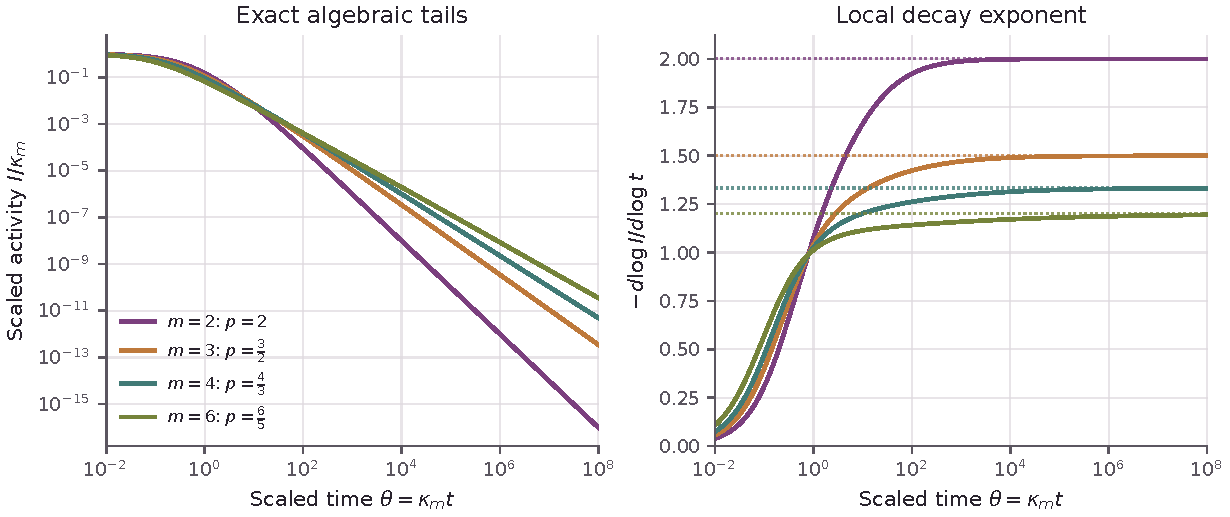
\includegraphics[width=1\linewidth,height=\textheight,keepaspectratio,alt={Numerical evaluations of the exact scalar quadrature for the constructed family. Time is rescaled as \textbackslash theta=\textbackslash kappa\_m t, and activity as I/\textbackslash kappa\_m. The right panel evaluates the analytic local log-log slope; dotted levels are m/(m-1).}]{figures/decay_family.pdf}
\caption{Numerical evaluations of the exact scalar quadrature for the
constructed family. Time is rescaled as \(\theta=\kappa_m t\), and
activity as \(I/\kappa_m\). The right panel evaluates the analytic local
log-log slope; dotted levels are \(m/(m-1)\).}
\end{figure}

\section{4. Four states are necessary}\label{four-states-are-necessary}

We first reproduce the structural facts needed for a self-contained
lower bound on dimension.

\textbf{Lemma 4.} Under (T), every state fraction has a limit and every
channel flux has a finite integral. Under (T) and (D), every vanishing
state is integrable and has a persistent dependency successor.

\textbf{Proof.} Topologically label the states \(1,\ldots,n\). Every
prefix mass \(\sum_{i\le j}y_i\) is nonincreasing, so all coordinate
limits exist. The nonnegative potential \[
V(t)=\sum_{i=1}^n(n-i)y_i(t)
\] decreases by \((j-i)\) times the flux of a channel \(i\to j\). Hence
\(-V'\) dominates the sum of all channel fluxes, which proves their
integrability.

Let \(\mathcal A\) contain the vanishing states with infinite time
integral. No vertex of \(\mathcal A\) can have a persistent dependency
successor: such a successor would give outflow at least \(c y_i\)
eventually, contradicting the finite flux integral. Every vertex of
\(\mathcal A\) must nevertheless have a nonintegrable dependency
successor. Indeed, with outflow hazard
\(h_i(t)=\sum_k\beta^i_{ik}y_k(t)\), one has \[
y_i(t)\ge y_i(0)\exp\left(-\int_0^t h_i(s)\,ds\right).
\tag{19}
\] If all successors were integrable, this lower bound would stay
positive. A nonintegrable successor cannot be persistent by the
preceding observation, so it belongs to \(\mathcal A\). Following these
edges produces a cycle with no vertex having a persistent successor,
contrary to (D). Thus \(\mathcal A\) is empty. Applying (19) again shows
that every vanishing state must have a persistent successor. Persistent
states cannot have persistent successors because the associated channel
flux would tend to a positive constant. \(\square\)

\textbf{Theorem 5 (sharp minimum dimension).} Under (T), (D), and
strictly positive initial fractions, every vanishing state in a model
with at most three states admits an exponential upper bound. The
four-state example in Theorem 1 is therefore minimal.

Here the number of states counts population compartments in the channel
model; it is not the dimension after eliminating conservation laws.

\textbf{Proof.} For three states, take a topological order \((x,y,z)\).
The final state \(z\) is a transition sink and persists. If \(x\)
vanishes, Lemma 4 supplies a persistent dependency successor. Since
\(x\) has no inflow, \(\dot x\le-cx\) eventually. If \(y\) also
vanishes, its only possible persistent successor is \(z\), and its
inflow is bounded by \(Mx\). Hence \(\dot y\le Mx-c'y\) eventually, for
\(c,c'>0\). Variation of constants gives an exponential upper bound; any
resonant factor \(t\) is absorbed by a slightly smaller exponent.

It remains to treat \(x\to x^*>0\) and \(y\to0\). A
persistent-to-persistent channel flux cannot have a positive limit.
Since \(x\) has no inflow, its outflow must therefore be \(\alpha xy\).
Its contribution to the inflow of \(y\) is \(\beta xy\), with
\(0\le\beta\le\alpha\). Write the outflow from \(y\) as
\(y(\gamma x+\epsilon y+\delta z)\), with nonnegative coefficients.
After using \(z=1-x-y\), the exact two-coordinate equations are \[
\dot x=-\alpha xy,\qquad
\dot y=y[dx-\delta+ey],
\quad d=\beta-\gamma+\delta,\quad e=\delta-\epsilon.
\tag{20}
\] If \(\alpha=0\), then \(\beta=0\), so \(y\) has no inflow and its
persistent successor gives exponential decay. Suppose \(\alpha>0\). The
limiting per-capita growth rate is \(\ell=dx^*-\delta\). A positive
\(\ell\) contradicts \(y\to0\), and a negative \(\ell\) gives
exponential decay directly. We exclude \(\ell=0\).

Under that equality \(d=\delta/x^*\ge0\). Since \(x\) strictly decreases
to \(x^*>0\), write the positive orbit as \(y=Y(x)\) for \(x>x^*\).
Dividing (20) and using \(Y(x^*)=0\) gives \[
Y'(x)+\frac e{\alpha x}Y(x)
=-\frac d{\alpha x}(x-x^*).
\] The coefficients are regular at \(x^*\). Multiplication by
\(x^{e/\alpha}\) and integration yield \[
Y(x)=-\frac d\alpha x^{-e/\alpha}
\int_{x^*}^{x}s^{e/\alpha-1}(s-x^*)\,ds\le0,
\tag{21}
\] contradicting positivity, including when \(d=0\). Thus \(\ell<0\).

With two states a vanishing state is a source, and the source-state
argument applies. With one state no state vanishes. \(\square\)

\section{5. The complete four-state extinction
boundary}\label{the-complete-four-state-extinction-boundary}

The algebraic trajectory lies on a precise critical surface. This limits
any claim of robustness and supplies a direct sensitivity calculation.

For arbitrary positive initial fractions in (3), define \[
K=I_0+X_0-Y_0,\qquad B=2Y_0-X_0,\qquad
\Delta=B^2-4Y_0I_0.
\tag{22}
\] The same internal time gives \[
X=X_0u,\quad Y=Y_0u^2,\quad
I=F(u)=K-X_0u+Y_0u^2,\qquad \dot u=-uF(u).
\tag{23}
\]

\textbf{Theorem 6 (phase classification).} Exactly one of the following
occurs.

\begin{enumerate}
\def\labelenumi{\arabic{enumi}.}
\tightlist
\item
  If \(B>0\) and \(\Delta>0\), then \(I\) vanishes exponentially. With
  \[
  q=\frac{X_0+\sqrt\Delta}{2Y_0}\in(0,1),\qquad
  \lambda=q\sqrt\Delta>0,
  \] one has \(u-q\sim c e^{-\lambda t}\) and
  \(I\sim c\sqrt\Delta e^{-\lambda t}\) for some \(c>0\).
\item
  If \(B>0\) and \(\Delta=0\), then \(q=X_0/(2Y_0)\in(0,1)\),
  \(K=Y_0q^2>0\), and \[
  I(t)\sim\frac1{Kt^2},\qquad \int_0^\infty I(t)\,dt=-\log q.
  \]
\item
  In every other case, \(K>0\) and \(I\to K\). For some \(c>0\),
  \(X\sim X_0c e^{-Kt}\) and \(Y\sim Y_0c^2e^{-2Kt}\).
\end{enumerate}

In cases 1 and 2 the limit is \((X_0q,Y_0q^2,0,1-X_0q-Y_0q^2)\); in case
3 it is \((0,0,K,1-K)\). Both (T) and (D) hold in all three cases.

\textbf{Proof.} The quadratic \(F\) is positive at one and has positive
leading coefficient. A first root in \((0,1)\), approached as \(u\)
decreases, exists exactly when its vertex lies below one and its
discriminant is nonnegative. These are \(B>0\) and \(\Delta\ge0\). For
\(\Delta>0\), the first root is the larger root \(q\) and
\(F'(q)=\sqrt\Delta\). Separation of (23) gives the positive exponential
equivalent in case 1. For \(\Delta=0\), \(F(u)=Y_0(u-q)^2\);
differentiating \(1/(u-q)\) proves case 2.

If no root occurs in \((0,1)\), then \(u\to0\). Necessarily \(K>0\): a
negative \(K\) forces an intervening root, while \(K=0\) makes
\(F(u)=u(Y_0u-X_0)\) negative for small positive \(u\). Now
\(\dot u=-Ku+O(u^2)\) gives \(u\sim c e^{-Kt}\). The limits follow from
(23) and conservation. In extinction cases the cycle
\(Y\leftrightarrow I\) has persistent successor \(Y\) from \(I\); in the
persistence case it has persistent successor \(I\) from \(Y\).
\(\square\)

For \(X_0=Y_0=2/9\), the exact threshold is \(I_0=1/18\). Values
\(I_0=1/36,1/18,1/12\), with \(R_0\) adjusted to keep total mass one,
lie respectively below, on and above the threshold. The graph is
identical in all three cases. The critical equality is one equation in
the initial fractions, so arbitrary perturbations need not preserve the
algebraic tail. Multiplying every rate by a common positive constant
changes the time unit and preserves the exponent.

\section{6. An exact spectral repair}\label{an-exact-spectral-repair}

The graph conditions do not account for cancellation between limiting
inflow and outflow. A transverse Jacobian does. The following statement
uses (T) alone.

For a trajectory with limit \(y^*\), let \(V=\{i:y_i^*=0\}\) be nonempty
and \(P\) its complement. Put \(v=y_V\), \(p=y_P\), and \[
A=\left(\frac{\partial F_i}{\partial y_j}(y^*)\right)_{i,j\in V}.
\tag{24}
\] A matrix is \textbf{Metzler} when its off-diagonal entries are
nonnegative and \textbf{Hurwitz} when all its eigenvalues have strictly
negative real parts. Write
\(s(A)=\max\{\Re\lambda:\lambda\in\sigma(A)\}\).

\textbf{Theorem 7 (spectral equivalence).} Under (T) and strictly
positive initial fractions, \(A\) is Metzler and \(s(A)\le0\). Every
vanishing coordinate admits an exponential upper bound if and only if
\(s(A)<0\). In that case the entire trajectory converges exponentially
to \(y^*\).

\textbf{Proof.} Lemma 4's first part uses only (T). Each channel flux is
integrable and tends to its value at \(y^*\), so that limiting value is
zero. Consequently every nonzero channel contains at least one factor
indexed by \(V\). Thus, for a constant \(C\),
\(\|p'(t)\|_1\le C\|v(t)\|_1\). The negative terms in \(F_i\) all
contain \(y_i\), so the transverse matrix has nonnegative off-diagonal
entries.

Separate terms linear in \(v\), whose other factor belongs to \(p\),
from quadratic terms in \(v\). Since every \(p_k^*>0\), there are a
positive diagonal matrix \(D\) and a nonnegative function
\(\eta(t)\to0\) such that, componentwise for large \(t\), \[
v'\ge\bigl(A-\eta(t)A_{\mathrm{off}}-\eta(t)D\bigr)v.
\tag{25}
\] Here \(A_{\mathrm{off}}\) has the off-diagonal entries of \(A\) and
zero diagonal. Indeed, choose \(\eta\) to dominate
\(\max_k|p_k/p_k^*-1|\) and \(\|v\|_1\). Each positive off-diagonal
linear coefficient is at least \((1-\eta)\) times its limit. Changes in
diagonal linear terms and all negative quadratic terms are bounded by a
fixed diagonal multiple of \(\eta\); positive quadratic terms may be
discarded. Increasing \(D\) proves (25). If \(v\) decays exponentially,
integration of the bound on \(p'\) also gives exponential decay of
\(p-p^*\), so \(\eta\) can be chosen integrable.

Suppose \(s(A)>0\). For sufficiently small fixed \(\xi>0\), the Metzler
matrix \(A_{\xi}=A-\xi A_{\mathrm{off}}-\xi D\) has positive spectral
bound. Eventually \(v'\ge A_{\xi}v\). A nonnegative nonzero left Perron
vector \(w\) of \(A_{\xi}\) gives \((w^Tv)'\ge s(A_{\xi})w^Tv\). Strict
positivity of \(v\) implies \(w^Tv>0\), contradicting \(v\to0\). Thus
\(s(A)\le0\).

If \(s(A)<0\), choose a strictly positive row vector
\(w^T=\mathbf1^T(-A)^{-1}\), so \(w^TA=-\mathbf1^T\). The inverse is
nonnegative, for example from \((-A)^{-1}=\int_0^\infty e^{At}\,dt\),
and its diagonal entries are positive. Polynomial expansion yields
\(v'=Av+r(t)\) with \(\|r(t)\|_1=o(\|v(t)\|_1)\). Consequently
\((w^Tv)'\le-cw^Tv\) eventually for some \(c>0\). This gives exponential
bounds for \(v\), and then for \(p-p^*\).

Finally suppose \(s(A)=0\) and every vanishing coordinate decays
exponentially. Take a nonnegative nonzero left Perron vector \(w\) with
\(w^TA=0\) and put \(q=w^Tv>0\). Since
\(w^TA_{\mathrm{off}}=-w^T\operatorname{diag}(A)\), equation (25) gives
\[
q'\ge-\eta(t)\sum_iw_i(D_{ii}-A_{ii})v_i
\ge-L\eta(t)q
\tag{26}
\] for a fixed positive \(L\). Integrability of \(\eta\) then gives a
strictly positive lower bound on \(q(t)\), contradicting \(q\to0\). This
excludes \(s(A)=0\) under exponential extinction. \(\square\)

Metzler transverse Jacobians and strict spectral sufficient conditions
are established tools in positive systems and boundary-stability theory
{[}6-9{]}. Wiersdalen et al.~{[}6, Theorem 2{]} give an
attraction-versus-exponential-stability equivalence for a compartmental
base matrix and compartmental perturbations preserving its zero
off-diagonal and column-sum pattern. Johnston and Avram {[}7, Theorem
1{]} obtain local boundary-stability tests from strict
reproduction-number inequalities. Adenane, Avram and Halanay {[}8,
Theorems 6-7{]} study spectral thresholds and local boundary
bifurcations, with a Hurwitz tangential block and nondegenerate crossing
conditions for the bifurcation result. Related balanced bilinear
epidemic models are treated in {[}9{]}.

The specific additional assertion here is the necessity of a strict
transverse spectral gap for exponential approach along an initially
positive trajectory in the acyclic channel class, including reducible
transverse blocks. Every channel vanishes on the limiting persistent
face, whose tangential dynamics are identically zero; the critical
constructions therefore do not satisfy the tangential stability
hypothesis of {[}8{]}. Our transverse matrix need not be compartmental,
and the proof imposes no zero-pattern restriction on an additive
perturbation. The criterion depends on the particular limiting state and
supplies no graph-only procedure for determining it. We do not claim
novelty for Metzler structure, positive-matrix comparison or the
sufficiency of a Hurwitz block.

\textbf{Corollary 8 (exact logarithmic extinction rate).} Under the
hypotheses and notation of Theorem 7, \[
\lim_{t\to\infty}\frac{\log\|v(t)\|_1}{t}=s(A).
\tag{27}
\] Thus a zero spectral bound means that the total vanishing population
has zero exponential rate, not merely that one chosen exponential
estimate fails. If \(s(A)<0\), the same limit holds with
\(\|y(t)-y^*\|_1\) in place of \(\|v(t)\|_1\). These are logarithmic
rates; they do not assert a pure exponential equivalent or a common rate
for each coordinate.

\textbf{Proof.} Fix \(0<\varepsilon<1\). The lower comparison in (25)
eventually gives \[
v'\ge A_\varepsilon v,\qquad
A_\varepsilon=A-\varepsilon A_{\mathrm{off}}-\varepsilon D.
\] A nonnegative nonzero left Perron vector \(w_\varepsilon\) satisfies
\(w_\varepsilon^TA_\varepsilon=s(A_\varepsilon)w_\varepsilon^T\). Since
\(v\) is strictly positive, integration of the resulting scalar
inequality gives
\(\liminf_{t\to\infty}t^{-1}\log\|v(t)\|_1\ge s(A_\varepsilon)\). For
the upper bound, the remainder estimate in Theorem 7 gives
\(|r_i(t)|\le\|r(t)\|_1\le\varepsilon\|v(t)\|_1\) eventually for every
\(i\). Hence \[
v'\le B_\varepsilon v,\qquad
B_\varepsilon=A+\varepsilon\mathbf1\mathbf1^T.
\] The Metzler matrix \(B_\varepsilon\) has strictly positive
off-diagonal entries (and the scalar case is immediate), so its left
Perron vector can be chosen strictly positive. Its pairing with \(v\) is
therefore comparable to \(\|v\|_1\), and the upper scalar inequality
yields \(\limsup_{t\to\infty}t^{-1}\log\|v(t)\|_1\le s(B_\varepsilon)\).
Continuity of the spectral bound as \(\varepsilon\downarrow0\) proves
(27), including for reducible \(A\).

If \(s(A)<0\), for every \(\delta>0\) with \(s(A)+\delta<0\) the upper
comparison gives \(\|v(t)\|_1\le C_\delta e^{(s(A)+\delta)t}\)
eventually. Integrating \(\|p'\|_1\le C\|v\|_1\) from \(t\) to infinity
gives the same upper rate for \(\|p-p^*\|_1\). The lower rate follows
from \(\|y-y^*\|_1\ge\|v\|_1\). Letting \(\delta\downarrow0\) completes
the proof. \(\square\)

This corollary is a direct sharpening of the same positive-matrix
comparison, not a claim to a new general theory of asymptotically linear
systems. It is useful because it gives a precise aggregate rate even
when the transverse block is reducible. Strict initial positivity
remains essential: an identically absent coordinate can fail to excite
the slow spectral mode.

In the four-state model, \(A=[-\lambda]\) in the exponential-extinction
regime, \(A=[0]\) on the critical boundary, and
\(A=\operatorname{diag}(-K,-2K)\) when \(I\) persists and \(X,Y\)
vanish. The aggregate logarithmic rates are respectively \(-\lambda\),
\(0\), and \(-K\). In the family of Theorem 2 only \(I\) vanishes;
identity (17) gives its transverse eigenvalue zero.

\section{7. Verification, interpretation and
limits}\label{verification-interpretation-and-limits}

The executable \texttt{verify.py} uses only Python's standard library
and exact rational arithmetic. It constructs each ordinary differential
equation from the individual conversion channels, independently
constructs the closed-form polynomial trajectory, and checks equality of
every coefficient after differentiation. It also checks normalisation,
exact limits, transition acyclicity and condition (D). The latter is
checked by deleting all vertices with a persistent dependency successor
and testing the remaining induced graph for acyclicity. All 24 cases
\(m=2,\ldots,25\) pass. The three phase regimes are separately checked
against the channel equations. These finite checks detect algebraic and
transcription errors; they do not replace the proofs for arbitrary \(m\)
or the minimum-dimension theorem. The separate plotting script evaluates
the scalar quadrature using NumPy, SciPy and Matplotlib; these packages
are not required by the exact verifier.

The scalar time change explains the mechanism. For a positive activity
\(I\), the accumulated activity \(\tau=\int I\) makes the reservoir
equations linear. In Theorem 2, \(u=e^{-\tau}\) and \(I=C(u-q)^m\) for
\(q=1/2\). Physical time diverges when the internal-time activity
reaches its repeated zero. More generally, if an analytic scalar
reduction satisfies \[
\tau'=F(\tau),\qquad
F(\tau)=a(\tau^*-\tau)^m+o((\tau^*-\tau)^m),\quad a>0,
\] at a finite terminal internal time, a simple zero gives exponential
decay; an \(m\)-fold zero with \(m\ge2\) gives an activity proportional
to \(t^{-m/(m-1)}\). This is a scalar asymptotic calculation. The
construction shows that the required cancellations can occur inside the
original nonnegative quadratic channel class.

The result provides no fitted parameters, observed-population evidence
or recommendation for disease control. Its applied relevance is
mathematical: a modeller cannot use the two graph conditions alone to
justify an exponential tail, an exponential stopping rule or a
logarithmic extinction-time estimate. Under the exact family, reaching a
small activity threshold \(a\) instead takes asymptotically
\((K_m/a)^{1/p_m}\) time, whereas an exponential law would give
logarithmic growth in \(1/a\). Any practical use requires matching the
model, its parameters and its initial condition.

The four-state slow tail requires a critical equality. Higher
multiplicities impose further cancellations. We have proved existence
and exact consequences, not prevalence or robustness to arbitrary
perturbations. Theorem 7 supplies a strict spectral condition under
which exponential convergence does follow. The bounded search through 19
October 2026 found no earlier resolution of the source conjecture, but
cannot certify historical priority or exclude unindexed work. The proof
does not depend on such a priority claim.

\section{8. Availability and
declarations}\label{availability-and-declarations}

\textbf{Data and code availability.} This is a theoretical study with no
observational dataset. The accompanying repository contains this
manuscript, \texttt{verify.py}, \texttt{test\_verifier.py}, exact replay
receipts, the figure and its plotting source. The source repository is
\url{https://github.com/ipitchford/algebraic-extinction-compartments}
and the versioned archive is
\url{https://doi.org/10.5281/zenodo.23501636}. Running
\texttt{python3\ -B\ test\_verifier.py\ -\/-output-dir\ NEW\_DIRECTORY}
repeats the finite rational checks in normal and optimized Python modes
and requires three deliberate corruptions to be rejected in each mode.
The analytic proofs, rather than those finite checks, establish the
general results.

\textbf{Ethics.} No human participants, animal subjects or personal data
are involved. The models are mathematical constructions, not clinical or
policy recommendations.

\textbf{Contributions.} The release records conceptualisation, formal
analysis, software, validation, visualisation and writing. It is
presented anonymously; the supplied research record does not assign
these CRediT roles to named human contributors.

\textbf{Funding and competing interests.} No external grant funding or
competing interest is declared in the supplied research record. Evidence
Press publication does not constitute institutional or journal
endorsement.

\textbf{AI assistance and assurance.} AI assistants were used for
research development, proof criticism, code and manuscript preparation.
This revision used Codex for proof inspection, exposition, a
logarithmic-rate corollary and verification hardening, with a separate
AI check of the corollary. AI review is not external human peer review.
Exact arithmetic replay is not proof-assistant formal verification, and
the bounded literature search does not certify historical priority.

\section{References}\label{references}

\subsection{Originating conjecture}\label{originating-conjecture}

{[}1{]} Chan, K. M. D., Crommelin, D. T., \& Mandjes, M. R. H. (2025).
\emph{Asymptotic behavior for a general class of spreading models}
{[}Preprint{]}. arXiv. \url{https://doi.org/10.48550/arXiv.2511.02437} .
Inspected mathematical text: \url{https://arxiv.org/html/2511.02437v1} ;
institutional copy: \url{https://ir.cwi.nl/pub/36026/} . The
bibliographic year follows the arXiv submission record; the exact
conjecture is identified by section and number.

\subsection{Algebraic decay and kinetic
representations}\label{algebraic-decay-and-kinetic-representations}

{[}2{]} Luhar, M., Oberai, A. A., Fokas, A. S., \& Yortsos, Y. C.
(2022). Accounting for super-spreader events and algebraic decay in SIR
models. \emph{Computer Methods in Applied Mechanics and Engineering,
401}, 115286. \url{https://doi.org/10.1016/j.cma.2022.115286}

{[}3{]} Craciun, G., Johnston, M. D., Szederkényi, G., Tonello, E.,
Tóth, J., \& Yu, P. Y. (2020). Realizations of kinetic differential
equations. \emph{Mathematical Biosciences and Engineering, 17}(1),
862-892. \url{https://doi.org/10.3934/mbe.2020046}

\subsection{Established analytical methods and stability
criteria}\label{established-analytical-methods-and-stability-criteria}

{[}4{]} Harko, T., Lobo, F. S. N., \& Mak, M. K. (2014). Exact
analytical solutions of the Susceptible-Infected-Recovered (SIR)
epidemic model and of the SIR model with equal death and birth rates.
\emph{Applied Mathematics and Computation, 236}, 184-194.
\url{https://doi.org/10.1016/j.amc.2014.03.030}

{[}5{]} Damianou, P. A., \& Petalidou, F. (2014). On the liouville
intergrability of Lotka-Volterra systems. \emph{Frontiers in Physics,
2}, Article 50. \url{https://doi.org/10.3389/fphy.2014.00050} (Title
spelling follows the publisher.)

{[}6{]} Wiersdalen, S., Pereira, M., Lang, A., Szederkényi, G., Auriol,
J., \& Kulcsár, B. (2026). Linear Lyapunov functions for nonlinear
compartmental systems. \emph{IEEE Transactions on Automatic Control}.
Advance online publication.
\url{https://doi.org/10.1109/TAC.2026.3708062} . Inspected preprint:
\url{https://arxiv.org/pdf/2312.11061v3}

{[}7{]} Johnston, M. D., \& Avram, F. (2026). The boundary reproduction
number for determining boundary steady state stability in chemical
reaction systems. \emph{Journal of Mathematical Biology, 92}, Article
29. \url{https://doi.org/10.1007/s00285-026-02351-z} . Inspected author
preprint: \url{https://arxiv.org/pdf/2506.01606}

{[}8{]} Adenane, R., Avram, F., \& Halanay, A.-D. (2026). Persistence,
coexistence, and boundary transcritical relays for multi-strain epidemic
models. \emph{Mathematics, 14}(18), Article 3271.
\url{https://doi.org/10.3390/math14183271} . Inspected author preprint:
\url{https://www.preprints.org/manuscript/202608.0347} . The comparison
refers to Theorems 6-7 of this accessible preprint; the publisher record
was also checked.

{[}9{]} Adenane, R., Avram, F., Halanay, A.-D., Horvath, A., \& Khong,
S. Z. (2026). A Perron-Frobenius strong threshold theorem for
\((A,B,P,\varphi)\) balanced bilinear model. \emph{Mathematical
Biosciences and Engineering, 23}(9), 2720-2770.
\url{https://doi.org/10.3934/mbe.2026098} . Published author order and
metadata follow the publisher; the inspected author preprint,
\url{https://arxiv.org/pdf/2605.24629}, has a different title and author
order.

\end{document}
